\section{Filter Creation}
Before creating any HDL code, the filter has to be normally implemented in MATLAB.
Using \verb|designfilt| command, every parameter of the filter is filled with the help of GUI. We call this function 3 times, one for each different order of filter, thus creating 3 different FIR filters.
\begin{figure}[htpb]
    \centering
    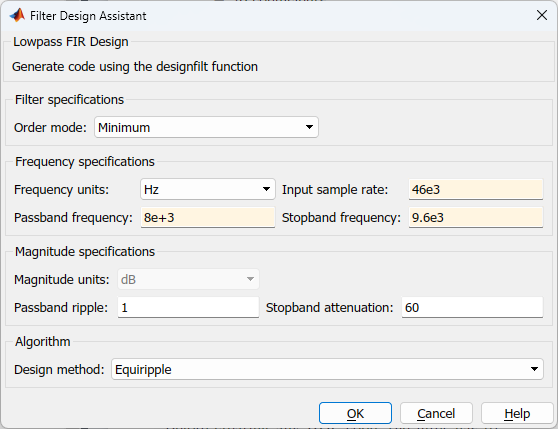
\includegraphics[width=0.4\textwidth]{Images/matlab_filter_design_assist_tool.png}
    \caption{MATLAB's design assist tool for creating lowpass FIR filters}
    \label{fig:matlab_filter_design_assist_tool}
\end{figure}
Using \verb|fvtool|, all three filters can be compared and be checked for compliance. 

For HDL Coder to work, all filters must be designed by \verb|fdesign.lowpass()| and \verb|design()| functions, thus all filters created above must be re-created. The first function creates the specification for each filter containing useful information such as passband/stopband frequency, sample rate, etc. In order to actually create the filter, \verb|design()| function has to be called and it returns \verb|dsp.FIRFilter| data type, meaning that the wanted filter is successfully created. Note that, we make use of two specific toolboxes provided by Mathworks, called \emph{DSP System Toolbox} and \emph{DSP HDL Toolbox} that provide those "easy" methods of creating filters alongside with optimizations like pipelining, CSD and others needed for this project. 

After each filter is created, \verb|fdhdltool| has to be called with filter specifications and numeric type needed as arguments.
Every aspect of the generated filter can be tuned from there such configuring architectures, multiplier pipelining, test bench generator and more. This task has to be executed for each implemented filter.

\begin{figure}[htbp]
    \centering
    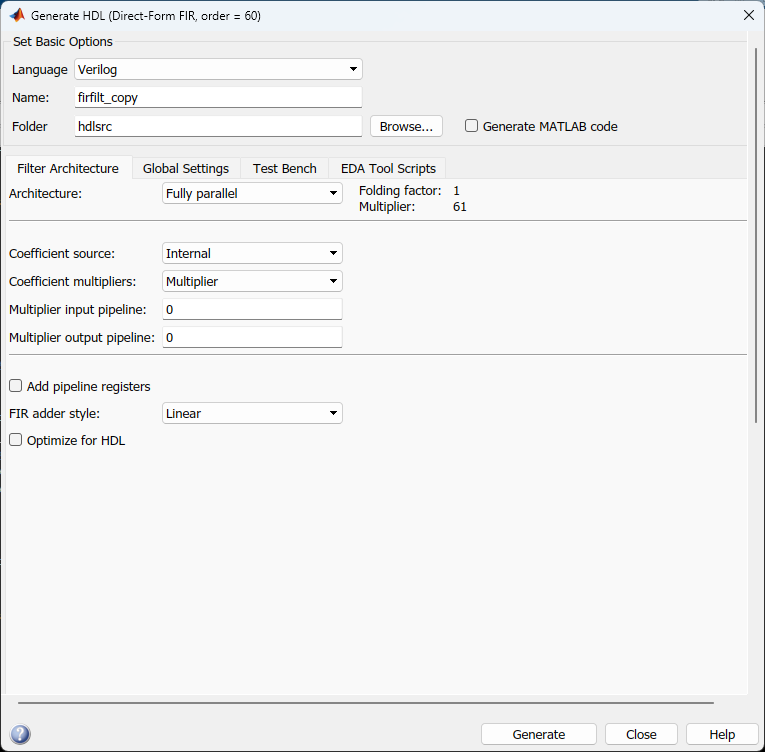
\includegraphics[width=0.4\textwidth]{Images/matlab_create_hdl.png}
    \caption{MATLAB's tool for creating HDL filters.}
    \label{fig:matlab_create_hdl}
\end{figure}
